\documentclass[12pt,letterpaper]{article}
\usepackage[latin1]{inputenc}
\usepackage{amsmath}
\usepackage{amsfonts}
\usepackage{amssymb}

% the above packages are the "base"

\usepackage{graphicx}
\graphicspath{{figs/}} % set the location of your figures

\usepackage{hyperref} % enable links within pdf
\hypersetup{colorlinks = true, linkcolor = black, urlcolor = blue}

\usepackage{float} % to fix the position of figures using [H]

% in-text citation styles
\usepackage[sort]{natbib}
\bibpunct[; ]{(}{)}{;}{a}{,}{;}

%  You "comment out" lines with the % symbol.

\author{}
\title{\textbf{This will be my awesome title.}\\An Intro to \LaTeX}


\begin{document}
\maketitle

\tableofcontents

\pagebreak


\section{Introduction}
\label{sec:intro} % labels allow automatic referencing

I think it's fair to say that most biologists switch from using word processors (like Microsoft Word or 
Apple Pages) to \LaTeX\ when they start writing papers containing more than just one or two equations.  I 
have to admit though, that after using both \LaTeX\ and Pages for a few years (depending on the type of 
manuscript I was writing), I've now switched entirely to writing manuscripts in \LaTeX\ (when 
collaborators allow).  It took me a while to get the hang of it, but now I prefer it even when there are no 
equations involved.

Note that (almost) all the lecture notes for this class were written in \LaTeX\, so take a look at a few of 
their \texttt{tex} files to learn a few additional tricks.

Note that your \LaTeX\ file is code that gets compiled.

\section{Basics}

\subsection{Document structure}
What isn't visible here in this pdf document is that the code for every \LaTeX\ document begins with a 
preamble that sets things up.  
In the preamble you define the type of document it is, load necessary 
packages, define any additional functions you might like to have, and provide your author name and the 
title of the paper.  
Your actual text is then written after beginning your document  using 
\verb+\begin{document}+ and is followed at the very end by \verb+\end{document}+.\footnote{Many 
	other functions use the same  begin $\ldots$ end structure.}

You "comment out" lines with the \% symbol.
Also, if you look at the raw \texttt{.tex} file behind this pdf, you'll notice that I wrote each sentence on its 
own line (i.e. with hard-returns between each).
That's not necessary, but allows \texttt{Git} to distinguish changes on a sentence-specific rather than 
whole paragraph basis.
A common alternative is to setup your editor such that all lines are limited to 72 or 80 characters.


\subsection{Basic equations}

The fundamental principle of calculus entails
\begin{equation}
	\label{eqn:calculus}
	\lim_{{\Delta t} \to 0}\frac{f(a+\Delta t)-f(a)}{\Delta t}.
\end{equation}
Although the typical way of writing a derivative is $\frac{dx}{dt}$, some fields also write it as $\dot{x}$.

\subsection{Lists}
\noindent % if you don't want a particular section to auto-indent
Calculus rocks because it can be used to represent all of the following:
\begin{itemize}
	\item first item
	\item second item
\end{itemize}
It also rocks because
\begin{enumerate}
	\item first item
	\item second item
\end{enumerate}

\subsection{Tables}
One could also organize all the things calculus can be used for in a table:
\begin{center}
\begin{tabular}{lc} % {lc} means the 1st column is left-aligned while the 2nd is centered
		\hline
		\hline
		Reason & Explanation\\  % the \\ is  a "return/next line"
		\hline
			1 & blah blah blah \\
			2 & blah blah blah \\
		\hline
		\hline
	\label{tab:mytable}
\end{tabular}
\end{center}


\subsection{Within-text referencing}
I can easily reference the section (sect.\ref{sec:intro}), equation (eqn. \ref{eqn:calculus}) and table (Table \ref{tab:mytable}).
Their numbers will auto-generate, which makes it easy to move them around in your paper and adhere to 
a journal's stylistic preferences.

\subsection*{My un-numbered subsection}
Sections and subsection are numbered by default, but that can be overwritten for a given section, or 
globally using \verb+\setcounter{secnumdepth}{0}+ in the preamble.



\section{More equations}

\subsection*{Using align}
The Lotka-Voltera equations are given by
\begin{align}
\frac{dx}{dt} 	&=	\alpha x - \beta xy \\
\frac{dy}{dt}	&=	\gamma xy - \delta y
\end{align}

Often it's useful to typeset the steps of derivations. 
Pay it forward to folks who are trying to learn these 
methods, and to yourself when you can't remember the details but have to lecture on it in 5 minutes.
In these cases you don't need to number each line.

\begin{align}
N(10) 	&= 	\lambda N(9) 		\\ 		\notag
		&= 	\lambda^2 N(8) 	\\		\notag
		&=	\lambda^3 N(7) 	\\		\notag
		& \dots				\\		\notag
		&=	\lambda^{10} N(0)	\\		\notag
\end{align}


\section{Inserting figures}
Note that the position of figures is auto-determined (e.g., Fig.~\ref{fig:logo})!
You can force the position of figures using the \texttt{float} package and then the [H] option for your 
figure 
(e.g., Fig.~\ref{fig:miktex}).

% Figures are included like this:
\begin{figure}
	\centering
	
\includegraphics[width=0.2\linewidth]{LaTeX_logo.png}
	\caption{This is the \LaTeX~logo.}
	\label{fig:logo}
\end{figure}

\begin{figure}[H]
	\centering
	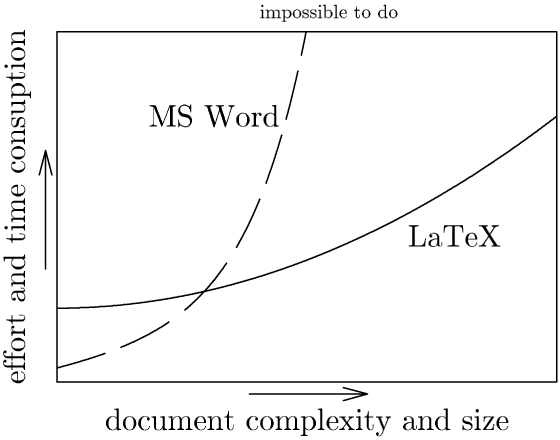
\includegraphics[width=0.8\linewidth]{figs/miktex.png}
	\caption{Why use \LaTeX\ (source: \url{http://www.pinteric.com/miktex.html})}
	\label{fig:miktex}
\end{figure}


\section{Intserting external tables}
It's relatively easy to use the R \texttt{Hmisc} package to generate \LaTeX\ tables (see 
\texttt{../R/ExportTable.R}) and then import them into your document using \texttt{input}.
Again, just like figures, their placement in the document is auto-determined.
If you provided a caption to the tables when generating their tex files in R, it's easy to reference them 
(Table \ref{tab:data} and \ref{tab:coefs}).


% Table created by stargazer v.5.2.3 by Marek Hlavac, Social Policy Institute. E-mail: marek.hlavac at gmail.com
% Date and time: Tue, Dec 10, 2024 - 16:53:33
\begin{table}[!htbp] \centering 
  \caption{} 
  \label{tab:data} 
\begin{tabular}{@{\extracolsep{5pt}}lccccc} 
\\[-1.8ex]\hline 
\hline \\[-1.8ex] 
Statistic & \multicolumn{1}{c}{N} & \multicolumn{1}{c}{Mean} & \multicolumn{1}{c}{St. Dev.} & \multicolumn{1}{c}{Min} & \multicolumn{1}{c}{Max} \\ 
\hline \\[-1.8ex] 
x & 6 & 0.601 & 0.387 & 0.098 & 0.980 \\ 
y & 6 & 3.211 & 1.732 & 0.872 & 4.533 \\ 
\hline \\[-1.8ex] 
\end{tabular} 
\end{table} 


% Table created by stargazer v.5.2.3 by Marek Hlavac, Social Policy Institute. E-mail: marek.hlavac at gmail.com
% Date and time: Tue, Dec 10, 2024 - 16:59:52
\begin{table}[!htbp] \centering 
  \caption{} 
  \label{tab:coefs} 
\begin{tabular}{@{\extracolsep{5pt}} ccccc} 
\\[-1.8ex]\hline 
\hline \\[-1.8ex] 
 & Estimate & Std. Error & t value & Pr(\textgreater \textbar t\textbar ) \\ 
\hline \\[-1.8ex] 
(Intercept) & $1.066$ & $0.381$ & $2.795$ & $0.012$ \\ 
x & $3.401$ & $0.655$ & $5.195$ & $0$ \\ 
\hline \\[-1.8ex] 
\end{tabular} 
\end{table} 



\section{References}

\begin{figure}
	\centering
	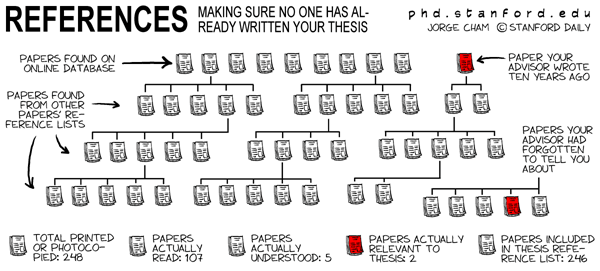
\includegraphics[width=1\linewidth]{figs/phd022702s.png}
	\caption{Reading is fundamental (source: \url{http://phdcomics.com/comics/archive.php?comicid=286})}
	\label{fig:phdrefs}
\end{figure}

The \texttt{natbib} package is great for citing references.
Reformatting for a different journal is as easy as changing the arguments of a function.
How to cite references and include them in a bibliography is demonstrated in the accompanying 
\texttt{manuscript.tex} template in the parent folder of these lecture notes.

\end{document}
